\chapter{Fisiologia Renal e Osmorregulação}\label{ch:b3:renal-osmoregulation}

Seus rins filtram cento e oitenta litros de plasma por dia --- todo o
seu volume de sangue a cada meia hora --- e devolvem tudo menos um litro
e meio, tendo retirado a ureia, ajustado o sal, o ácido e a água a menos
de um por cento do que o corpo precisa, e guardado cada grama de
glicose. Um rato-canguru do deserto nunca bebe: vive da água que seu
metabolismo faz a partir de sementes secas e excreta uma urina cinco
vezes mais concentrada que a água do mar. Um peixe marinho bebe sem
parar e bombeia o sal para fora pelas brânquias; um peixe de água doce
nunca bebe e bombeia sal para dentro. O problema que todos resolvem é o
mesmo: manter constante a composição do líquido em torno das células
enquanto comer, beber e respirar a perturbam, e descartar nitrogênio sem
descartar água demais. Este capítulo trata do rim dos mamíferos como
exemplo trabalhado --- a filtração, a aritmética do clearance, o truque
da contracorrente que concentra a urina e os hormônios que ajustam os
botões --- e depois da variedade de soluções entre os animais.

\section{O problema}

\begin{definition}[Osmorregulação]\label{def:b3:renal-osmoregulation:problem}
\index{osmolaridade}\index{pressão osmótica}\index{líquido extracelular}\index{osmoconformador}\index{osmorregulador}
A \emph{osmolaridade} de uma solução é sua concentração total de
partículas dissolvidas (em osmoles por litro); ela fixa a \emph{pressão
osmótica}, $\Pi = cRT$ para soluções diluídas, que move a água através
de qualquer membrana que deixe passar água mas não soluto. Os líquidos
corporais de um mamífero ficam em cerca de \qty{300}{mOsm/L} ---
\qty{40}{\%} da massa corporal dentro das células, \qty{20}{\%} fora, o
\emph{líquido extracelular}, do qual um quarto é plasma --- e as células
incham ou murcham em segundos se o lado de fora muda, já que suas
membranas deixam a água passar livremente. Um \emph{osmoconformador} (a
maioria dos invertebrados marinhos, os tubarões) mantém seus líquidos na
osmolaridade do mar e regula apenas sua composição; um
\emph{osmorregulador} (vertebrados, insetos, animais de água doce)
mantém sua osmolaridade constante contra o ambiente, o que custa energia
em proporção ao gradiente. A segunda tarefa, acoplada à primeira, é
livrar-se do nitrogênio da degradação de proteínas: como \emph{amônia},
em água abundante (peixes); como \emph{ureia}, solúvel e não tóxica, mas
que precisa de água para ser carregada (mamíferos); ou como \emph{ácido
úrico}, uma pasta excretada quase seca (aves, répteis, insetos).
\end{definition}

\section{O néfron e a filtração}

\begin{definition}[O néfron]\label{def:b3:renal-osmoregulation:nephron}
\index{néfron}\index{glomérulo}\index{túbulo proximal}\index{alça de Henle}\index{ducto coletor}
Cada rim humano abriga cerca de um milhão de \emph{néfrons}. O sangue
entra num \emph{glomérulo}, um tufo de capilares dentro da cápsula de
Bowman, cujas paredes --- endotélio fenestrado, membrana basal e os
diafragmas em fenda entre os pés dos podócitos --- deixam passar água e
todo soluto abaixo de cerca de \qty{60}{kDa}, mas retêm as proteínas e
as células. O filtrado corre pelo \emph{túbulo proximal}, que reabsorve
dois terços da água e do sal e toda a glicose e os aminoácidos; desce e
sobe a \emph{alça de Henle}, que penetra na medula e constrói o
gradiente de concentração da próxima seção; atravessa o \emph{túbulo
distal}, onde o sal é ajustado; e entra no \emph{ducto coletor}, onde o
conteúdo final de água é fixado pela vasopressina enquanto o ducto
atravessa a medula até a pelve. O sangue que sai do glomérulo entra num
segundo leito capilar em volta dos túbulos, que capta o que eles
reabsorvem.
\end{definition}

\begin{omfigure}
\begin{tikzpicture}[every node/.style={font=\scriptsize}, >=stealth]
  % cortex/medulla background
  \fill[omDef!6] (-0.5,0) rectangle (11.5,3.6); \fill[omProp!8] (-0.5,-3.4) rectangle (11.5,0);
  \node[right, gray] at (-0.4,3.4) {córtex}; \node[right, gray] at (-0.4,-3.2) {medula};
  % glomerulus
  \draw[thick, omThm, fill=omThm!20] (0.8,2.6) circle (0.55); \node[below, align=center] at (0.25,2.0) {glomérulo:\\filtração,\\\qty{180}{L/d}};
  % proximal tubule
  \draw[very thick, omDef] (1.35,2.6) .. controls (2.2,3.3) and (2.8,2.0) .. (3.2,2.6) .. controls (3.5,3.1) and (3.9,2.2) .. (4.2,2.6);
  \node[below, align=center] at (2.65,2.05) {túbulo proximal:\\\qty{67}{\%} do Na$^{+}$ e da água,\\toda a glicose, aminoácidos,\\HCO$_3^-$};
  % loop of Henle
  \draw[very thick, omDef] (4.2,2.6) -- (4.2,-2.8) arc[start angle=180, end angle=360, radius=0.4] -- (5.0,2.6);
  \node[left, align=right] at (4.1,-1.0) {ramo descendente:\\a água sai};
  \node[right, align=left] at (5.1,-1.6) {ramo ascendente:\\NaCl bombeado para fora,\\sem água};
  \node[right, align=left, omProp!80!black] at (5.1,-0.2) {\qty{25}{\%} do Na$^{+}$};
  % distal tubule
  \draw[very thick, omDef] (5.0,2.6) .. controls (5.4,3.2) and (6.0,2.0) .. (6.4,2.6) .. controls (6.8,3.1) .. (7.2,2.6);
  \node[above, align=center] at (6.0,3.1) {túbulo distal: Na$^{+}$ (aldosterona),\\Ca$^{2+}$, secreção de K$^{+}$};
  % collecting duct
  \draw[very thick, omMeth!70!black] (7.2,2.6) -- (7.8,2.6) -- (7.8,-3.2);
  \node[right, align=left] at (7.9,-1.2) {ducto coletor:\\água (vasopressina,\\aquaporina-2),\\ureia, H$^{+}$;\\\qty{1.5}{L/d} para fora};
  \draw[->, thick, omMeth!70!black] (7.8,-3.2) -- (7.8,-3.6);
  % osmolarity scale on the right
  \foreach \y/\c in {2.6/300, 0.0/600, -1.4/900, -2.8/1200} { \node[left, omProp!80!black, font=\tiny] at (11.4,\y) {\c\ mOsm}; }
  \draw[->, omProp!80!black] (11.4,2.9) -- (11.4,-3.1); \node[above, omProp!80!black, font=\tiny, align=center] at (11.4,3.0) {osmolaridade\\intersticial};
\end{tikzpicture}

{\small Um \omterm{def:b3:renal-osmoregulation:nephron}{néfron} estendido. Filtração no córtex; reabsorção em massa no
\omterm{def:b3:renal-osmoregulation:nephron}{túbulo proximal}; a \omterm{def:b3:renal-osmoregulation:nephron}{alça de Henle} mergulhando na medula, onde o
interstício fica mais salgado com a profundidade; o \omterm{def:b3:renal-osmoregulation:nephron}{ducto coletor}
atravessando de volta esse gradiente e cedendo água se a vasopressina
permitir.}
\end{omfigure}

\begin{theorem}[Filtração e clearance]\label{thm:b3:renal-osmoregulation:clearance}
\index{forças de Starling}\index{taxa de filtração glomerular}\index{clearance}\index{inulina}\index{creatinina}
O filtrado atravessa a parede glomerular a uma taxa fixada pelas
\emph{\omterm{thm:b3:renal-osmoregulation:clearance}{forças de Starling}}: a pressão hidrostática do capilar
$P_{\text{GC}}$ empurra o líquido para fora, a pressão hidrostática do
espaço de Bowman $P_{\text{BS}}$ e a pressão oncótica das proteínas
plasmáticas $\pi_{\text{GC}}$ o puxam de volta, e
\[
\text{GFR} = K_{f}\,\bigl(P_{\text{GC}} - P_{\text{BS}} - \pi_{\text{GC}}\bigr)
\approx K_{f}\,(55 - 15 - 30)\ \unit{mmHg} = K_{f}\times \qty{10}{mmHg},
\]
a \emph{\omterm{thm:b3:renal-osmoregulation:clearance}{taxa de filtração glomerular}}, cerca de \qty{125}{mL/min} num
adulto. Para qualquer substância $x$ com concentração plasmática
$P_{x}$, concentração urinária $U_{x}$ e fluxo de urina $V$, o
\emph{clearance}
\[
C_{x} = \frac{U_{x}\,V}{P_{x}}
\]
é o volume de plasma depurado de $x$ por unidade de tempo. Se $x$ é
livremente filtrado e nem reabsorvido nem secretado (a inulina, e quase
isso a creatinina), $C_{x} = \text{TFG}$; se é totalmente removido do
plasma que passa pelo rim (o para-aminohipurato em dose baixa), $C_{x}$
é igual ao fluxo plasmático renal; um clearance abaixo da TFG significa
reabsorção líquida; acima dela, secreção líquida; e a carga filtrada
$\text{TFG}
\times P_{x}$ menos a excreção $U_{x}V$ é a quantidade
reabsorvida.
\end{theorem}
\begin{proof}
A filtração é ultrafiltração através de uma parede porosa: o fluxo é
proporcional à pressão líquida que a atravessa, e a pressão líquida é a
hidrostática para fora menos a hidrostática e a oncótica para dentro
(Starling), sendo desprezível a pressão oncótica do filtrado, que não
tem proteína. Clearance: numa unidade de tempo o rim excreta $U_{x}V$ de
$x$; o volume de plasma que continha essa quantidade é $U_{x}V/P_{x}$.
Para uma substância apenas filtrada, o que é excretado é o que foi
filtrado, $\text{TFG}\times P_{x} = U_{x}V$, donde $C_{x} = \text{TFG}$.
Para uma totalmente extraída, todo o $x$ do plasma que passa,
$\text{FPR}\times P_{x}$, é excretado, donde $C_{x} = \text{FPR}$. O
balanço de massa dá a quantidade reabsorvida.
\end{proof}

\begin{example}[Clearances em números]\label{ex:b3:renal-osmoregulation:numbers}
Inulina infundida até um nível plasmático de \qty{1}{mg/mL} aparece na
urina a \qty{125}{mg/mL} com um fluxo de \qty{1}{mL/min}: $C = 125\times 1/1 =
\qty{125}{mL/min}$, a TFG, \qty{180}{L/d}. O para-aminohipurato
dá \qty{650}{mL/min}, o fluxo plasmático; com um hematócrito de $0.45$ o
fluxo sanguíneo renal é de \qty{1.2}{L/min}, um quinto do débito
cardíaco para \qty{0.5}{\%} da massa corporal, e a fração de filtração é
$125/650 = 0.19$. Ureia: plasma \qty{5}{mmol/L}, urina \qty{300}{mmol/L}
a \qty{1}{mL/min} --- clearance de \qty{60}{mL/min}, metade da TFG, de
modo que metade da ureia filtrada é reabsorvida. Glicose: clearance zero
em níveis plasmáticos normais, com cada molécula das \qty{180}{g}
filtradas por dia devolvida. A creatinina, produzida pelo músculo a uma
taxa constante e apenas filtrada, é a \omterm{met:b3:renal-osmoregulation:gfr}{medida da TFG} na clínica: quando a
TFG cai à metade, a creatinina plasmática dobra, sem coleta alguma de
urina.
\end{example}

\begin{method}[Medir a função renal]\label{met:b3:renal-osmoregulation:gfr}
\index{medida da TFG}
(1) Para um valor de pesquisa, infunda inulina até um nível plasmático
estável, colete urina cronometrada, meça os dois e calcule $UV/P$. (2)
Na clínica, meça a creatinina plasmática e estime a TFG a partir dela
com uma fórmula que corrija idade, sexo e tamanho corporal; a estimativa
é o que define os estágios da doença renal crônica (uma TFG abaixo de
\qty{60}{mL/min} por três meses). (3) Teste a seletividade do filtro
medindo a albumina na urina --- normalmente abaixo de \qty{30}{mg/d};
mais que isso significa uma barreira que vaza, o sinal mais precoce da
lesão renal do diabetes. (4) Teste a capacidade de concentração privando
de água durante a noite e medindo a \omterm{def:b3:renal-osmoregulation:problem}{osmolaridade} urinária, que deve
passar de \qty{800}{mOsm/L}; não conseguir concentrar com uma TFG normal
aponta para o \omterm{def:b3:renal-osmoregulation:nephron}{ducto coletor} ou para a vasopressina.
\end{method}

\begin{omfigure}
\begin{tikzpicture}
\begin{axis}[
  width=0.68\linewidth, height=5.6cm,
  axis x line=bottom, axis y line=left,
  xmin=0, xmax=800, ymin=0, ymax=700,
  xlabel={glicose plasmática (mg/dL)}, ylabel={mg/min},
  xlabel style={font=\small, at={(axis description cs:0.5,-0.12)}, anchor=north}, ylabel style={font=\small},
  tick label style={font=\small}, xtick={0,100,200,300,400,600,800}, ytick={0,200,375,600},
  clip=false,
]
\addplot[very thick, omDef, domain=0:800, samples=2] {1.25*x};
\addplot[very thick, omMeth!70!black, domain=0:200, samples=2] {1.25*x};
\addplot[very thick, omMeth!70!black, smooth] coordinates {(200,250) (250,300) (300,340) (350,365) (400,375) (800,375)};
\addplot[very thick, omThm, domain=0:180, samples=2] {0};
\addplot[very thick, omThm, smooth] coordinates {(180,0) (250,12) (300,35) (350,72) (400,125) (800,625)};
\draw[dashed, gray] (axis cs:180,0) -- (axis cs:180,700); \node[font=\scriptsize, gray, anchor=north west] at (axis cs:185,560) {limiar};
\draw[dashed, gray] (axis cs:0,375) -- (axis cs:800,375);
\node[font=\scriptsize, omDef, anchor=south east] at (axis cs:480,620) {filtrada: TFG $\times$ P};
\node[font=\scriptsize, omMeth!70!black, anchor=south west, align=left] at (axis cs:660,395) {reabsorvida:\\$T_{m} = \qty{375}{mg/min}$};
\node[font=\scriptsize, omThm, anchor=north west] at (axis cs:520,300) {excretada};
\end{axis}
\end{tikzpicture}

{\small A curva de titulação da glicose. A carga filtrada sobe com o
nível plasmático; os transportadores do \omterm{def:b3:renal-osmoregulation:nephron}{túbulo proximal} reabsorvem tudo
até seu máximo $T_{m}$; acima do limiar, em cerca de \qty{180}{mg/dL}
(\qty{10}{mmol/L}), a glicose transborda para a urina --- o açúcar na
urina do diabetes não tratado.}
\end{omfigure}

\section{Concentrar a urina}

\begin{proposition}[O multiplicador em contracorrente]\label{prop:b3:renal-osmoregulation:countercurrent}
\index{multiplicação em contracorrente}\index{efeito único}\index{vasopressina}\index{aquaporina}\index{reciclagem de ureia}
A \omterm{def:b3:renal-osmoregulation:nephron}{alça de Henle} constrói um gradiente de \omterm{def:b3:renal-osmoregulation:problem}{osmolaridade} de
\qty{300}{mOsm/L} no córtex a \qty{1200}{mOsm/L} na ponta da medula, sem
que célula alguma bombeie contra mais do que uma fração dele. O ramo
ascendente espesso bombeia NaCl de seu líquido para o interstício e é
impermeável à água, de modo que em cada nível deixa o interstício cerca
de \qty{200}{mOsm/L} mais salgado que seu próprio conteúdo --- o
\emph{\omterm{prop:b3:renal-osmoregulation:countercurrent}{efeito único}}. O ramo descendente é permeável à água e se
equilibra com o interstício, de modo que o líquido que desce fica mais
salgado à medida que desce e entrega à curva um líquido já concentrado,
do qual o ramo ascendente então bombeia; o líquido que sobe fica mais
diluído que o interstício em todos os níveis e deixa a alça a
\qty{100}{mOsm/L}, hipotônico. O fluxo em contracorrente converte um
pequeno efeito transversal num grande gradiente longitudinal: o líquido
mais salgado da curva foi feito de um líquido que já era salgado, etapa
sobre etapa. O \omterm{def:b3:renal-osmoregulation:nephron}{ducto coletor} então desce atravessando esse gradiente. Sem
\emph{vasopressina} (hormônio antidiurético) sua parede é impermeável à
água e um litro ou mais de urina diluída sai a cada hora; com ela, canais
de \emph{aquaporina-2} são inseridos na membrana luminal, a água sai pelo
gradiente para a medula, e a urina alcança a \omterm{def:b3:renal-osmoregulation:problem}{osmolaridade} da ponta,
\qty{1200}{mOsm/L}. A ureia, reabsorvida do ducto interno e retida na
medula, fornece metade da \omterm{def:b3:renal-osmoregulation:problem}{osmolaridade} da ponta, e os vasa recta, eles
próprios em contracorrente, removem a água reabsorvida sem lavar o
gradiente.
\end{proposition}

\begin{proof}[Evidência]
Wirz, Hargitay e Kuhn (1951) congelaram rins de rato e mediram o ponto
de fusão do líquido em fatias do córtex à papila: a \omterm{def:b3:renal-osmoregulation:problem}{osmolaridade} subia
continuamente com a profundidade, chegando ao valor da urina na ponta
--- o gradiente que a teoria do multiplicador em contracorrente (Kuhn,
um físico-químico, 1942) havia exigido. A micropunção dos túbulos
(Gottschalk, 1959) encontrou então o líquido da curva da alça hipertônico
e o que deixava o ramo ascendente hipotônico, com o líquido do \omterm{def:b3:renal-osmoregulation:nephron}{ducto
coletor} igualando o interstício em cada nível quando havia vasopressina.
Os roedores do deserto com as alças mais longas tinham os gradientes mais
íngremes e a urina mais concentrada.
\end{proof}

\begin{omfigure}
\begin{tikzpicture}[every node/.style={font=\scriptsize}, >=stealth]
  % loop
  \draw[very thick, omDef] (0,3.2) -- (0,-0.4) arc[start angle=180, end angle=360, radius=0.7] -- (1.4,3.2);
  \draw[very thick, omDef] (0.35,3.2) -- (0.35,-0.4) arc[start angle=180, end angle=360, radius=0.35] -- (1.05,3.2);
  % interstitial osmolarity bands
  \foreach \y/\c/\col in {2.8/300/10, 2.0/500/25, 1.2/700/40, 0.4/900/55, -0.4/1100/70, -1.0/1200/80} { \fill[omProp!\col, opacity=0.5] (-2.2,\y-0.4) rectangle (-0.2,\y+0.4); \node[left, font=\tiny] at (-2.25,\y) {\c}; }
  \node[left, align=right, font=\tiny] at (-2.25,3.35) {interstício\\(mOsm/L)};
  % arrows: water out of descending, NaCl out of ascending
  \foreach \y in {2.4,1.6,0.8,0.0} { \draw[->, thick, omDef!70!black] (0.15,\y) -- (-0.4,\y); }
  \node[left, omDef!70!black, font=\tiny] at (-0.45,2.4) {H$_2$O};
  \foreach \y in {2.4,1.6,0.8,0.0} { \draw[->, thick, omThm] (1.25,\y) -- (1.9,\y); }
  \node[right, omThm, font=\tiny] at (1.5,2.85) {NaCl bombeado};
  % fluid osmolarity labels inside limbs
  \node[above] at (0.17,3.25) {\qty{300}{} entra}; \node[above] at (1.22,3.25) {\qty{100}{} sai};
  \node[font=\tiny] at (0.7,-1.35) {1200 na curva};
  \node[below, align=center] at (0.2,-1.7) {ramo descendente: a água sai,\\o líquido concentra; ramo ascendente:\\o sal sai, o líquido dilui};
  % collecting duct
  \draw[very thick, omMeth!70!black] (4.2,3.2) -- (4.2,-1.4); \node[above, align=center] at (4.2,3.25) {ducto coletor};
  \foreach \y in {2.4,1.6,0.8,0.0,-0.8} { \draw[->, thick, omMeth!70!black] (4.1,\y) -- (3.5,\y); }
  \node[right, align=left, font=\tiny] at (4.3,1.2) {com vasopressina:\\aquaporina-2 inserida,\\a água sai pelo\\gradiente};
  \node[below, align=center] at (4.2,-1.5) {urina a\\\qty{1200}{mOsm/L}};
  % single effect note
  \node[right, align=left] at (6.4,2.6) {o efeito único: o ramo ascendente\\mantém o interstício $\sim\qty{200}{mOsm/L}$\\acima de seu próprio líquido em cada nível;\\o fluxo em contracorrente empilha os efeitos\\num gradiente de \qty{900}{mOsm/L}\\do córtex à papila};
\end{tikzpicture}

{\small O multiplicador em contracorrente. O sal bombeado do ramo
ascendente torna o interstício hipertônico; a água retirada do ramo
descendente concentra o líquido antes que ele chegue à bomba; o fluxo em
sentidos opostos empilha uma pequena diferença transversal num gradiente
de quatro vezes, que o \omterm{def:b3:renal-osmoregulation:nephron}{ducto coletor} usa para concentrar a urina quando a
vasopressina o abre à água.}
\end{omfigure}

\begin{proposition}[A aritmética da água]\label{prop:b3:renal-osmoregulation:water}
\index{perda hídrica obrigatória}\index{clearance de água livre}
Um corpo que precisa excretar uma carga diária de soluto $S$ (cerca de
\qty{600}{mOsm}, sobretudo ureia e sal) a uma \omterm{def:b3:renal-osmoregulation:problem}{osmolaridade} urinária
máxima $U_{\max}$ precisa de um volume mínimo de urina $V_{\min} = S/U_{\max}$: para um humano, $600/1200 = \qty{0.5}{L}$ por dia, a perda
hídrica \emph{obrigatória}, à qual os pulmões e a pele acrescentam cerca
de \qty{0.9}{L}. Beber água do mar (cerca de \qty{1000}{mOsm/L}, quase
tudo sal) fornece um litro de água com \qty{1000}{mOsm} de sal que
precisam ser excretados; em $U_{\max}$ isso consome $1000/1200 = \qty{0.83}{L}$ de urina, mas o sal é excretado junto com uma carga de
ureia, e o ganho líquido fica perto de zero ou negativo: um náufrago que
bebe água do mar se desidrata mais depressa que um que não bebe. O
\emph{\omterm{prop:b3:renal-osmoregulation:water}{clearance de água livre}}, $V - U_{\text{osm}}V/P_{\text{osm}}$, é o
volume de água sem soluto que o rim acrescenta ao corpo ou dele remove
por unidade de tempo: positivo numa sobrecarga de água (urina diluída),
negativo na desidratação.
\end{proposition}
\begin{proof}
O soluto sai apenas na urina (fora o suor), a uma concentração de no
máximo $U_{\max}$, de modo que $S = U V \le U_{\max}V$ dá $V \ge S/U_{\max}$. Para a água do mar: um litro traz \qty{1000}{mOsm};
excretá-los a \qty{1200}{mOsm/L} consome \qty{0.83}{L}, deixando
\qty{0.17}{L}, antes de contar os \qty{600}{mOsm} de soluto metabólico
do próprio dia, cuja excreção o consome. \omterm{prop:b3:renal-osmoregulation:water}{Clearance de água livre}: a
urina de volume $V$ e \omterm{def:b3:renal-osmoregulation:problem}{osmolaridade} $U_{\text{osm}}$ contém soluto
$U_{\text{osm}}V$, que ocuparia $U_{\text{osm}}V/P_{\text{osm}}$ na
\omterm{def:b3:renal-osmoregulation:problem}{osmolaridade} do plasma; o resto do volume é água em excesso disso,
removida do corpo.
\end{proof}

\begin{omfigure}
\begin{tikzpicture}
\begin{axis}[
  width=0.66\linewidth, height=5.4cm,
  axis x line=bottom, axis y line=left,
  xmin=0, xmax=1300, ymin=0, ymax=12,
  xlabel={osmolaridade urinária (mOsm/L)}, ylabel={volume de urina (L/dia)},
  xlabel style={font=\small, at={(axis description cs:0.5,-0.12)}, anchor=north}, ylabel style={font=\small},
  tick label style={font=\small}, xtick={50,300,600,1200}, ytick={0.5,2,6,12},
  clip=false,
]
\addplot[very thick, omDef, domain=50:1300, samples=100] {600/x};
\draw[dashed, gray] (axis cs:300,0) -- (axis cs:300,2); \draw[dashed, gray] (axis cs:1200,0) -- (axis cs:1200,0.5);
\node[font=\scriptsize, omDef, anchor=south west] at (axis cs:350,3.5) {$V = S/U$ com $S = \qty{600}{mOsm/d}$};
\node[font=\scriptsize, anchor=west, align=left] at (axis cs:1210,1.7) {concentração máxima:\\\qty{0.5}{L}};
\node[font=\scriptsize, anchor=south west] at (axis cs:60,9) {diluição máxima (\qty{50}{mOsm/L}): \qty{12}{L}};
\end{axis}
\end{tikzpicture}

{\small O volume de urina necessário para carregar o soluto de um dia,
em função de sua concentração. Da urina mais diluída que o rim consegue
fazer à mais concentrada, o volume varia por um fator de vinte e quatro;
a vasopressina escolhe o ponto.}
\end{omfigure}

\section{Regulação}

\begin{definition}[Os controles]\label{def:b3:renal-osmoregulation:controls}
\index{sistema renina--angiotensina--aldosterona}\index{aldosterona}\index{peptídeo natriurético atrial}\index{osmorreceptor}\index{retroalimentação tubuloglomerular}
Duas variáveis são reguladas separadamente: o \emph{volume} do \omterm{def:b3:renal-osmoregulation:problem}{líquido
extracelular}, que é uma questão de quanto sódio o corpo retém, e sua
\emph{\omterm{def:b3:renal-osmoregulation:problem}{osmolaridade}}, que é uma questão de água. Volume: as células do
aparelho justaglomerular, onde o túbulo distal toca a arteríola de seu
próprio \omterm{def:b3:renal-osmoregulation:nephron}{glomérulo}, liberam \emph{renina} quando a pressão arterial ou o
sal tubular caem; a renina cliva a angiotensina I de uma proteína
plasmática, a enzima conversora faz a \emph{angiotensina II}, que
contrai arteríolas, estimula a sede e libera \emph{aldosterona} do
córtex da adrenal, a qual, ao longo de horas, faz o túbulo distal e o
\omterm{def:b3:renal-osmoregulation:nephron}{ducto coletor} reabsorverem sódio (pelo canal ENaC) e secretarem
potássio. Os átrios distendidos liberam o \emph{peptídeo natriurético},
que faz o contrário. \omterm{def:b3:renal-osmoregulation:problem}{Osmolaridade}: \emph{osmorreceptores} do hipotálamo
percebem uma elevação de \qty{1}{\%} e liberam vasopressina da hipófise
posterior em minutos, e disparam a sede; uma queda a desliga. O rim
também se regula: a \emph{retroalimentação tubuloglomerular} contrai a
arteríola de um \omterm{def:b3:renal-osmoregulation:nephron}{néfron} cuja entrega distal de sal está alta demais,
mantendo a filtração de cada \omterm{def:b3:renal-osmoregulation:nephron}{néfron} dentro do que seu túbulo dá conta. E
o equilíbrio acidobásico: o \omterm{def:b3:renal-osmoregulation:nephron}{túbulo proximal} recupera o bicarbonato
filtrado, o \omterm{def:b3:renal-osmoregulation:nephron}{ducto coletor} secreta prótons contra um gradiente de mil
vezes e os excreta tamponados em fosfato e, acima de tudo, como amônio
feito a partir de glutamina --- a via pela qual o corpo se livra do
ácido de uma dieta rica em proteínas.
\end{definition}

\begin{omfigure}
\begin{tikzpicture}[every node/.style={font=\scriptsize}, >=stealth]
  \node[draw, thick, rounded corners, fill=omThm!20, align=center] (low) at (0,0) {pressão arterial baixa\\ou NaCl tubular baixo};
  \node[draw, thick, rounded corners, fill=omDef!20, align=center] (ren) at (3.6,0) {células justaglomerulares\\liberam renina};
  \node[draw, thick, rounded corners, fill=omDef!20, align=center] (ang) at (7.4,0) {angiotensina I $\to$ II\\(enzima conversora)};
  \node[draw, thick, rounded corners, fill=omMeth!25, align=center] (ald) at (11.0,1.2) {aldosterona:\\Na$^{+}$ retido, K$^{+}$ perdido};
  \node[draw, thick, rounded corners, fill=omMeth!25, align=center] (vc) at (11.0,-0.3) {arteríolas se contraem};
  \node[draw, thick, rounded corners, fill=omMeth!25, align=center] (th) at (11.0,-1.8) {sede, vasopressina};
  \draw[->, thick] (low) -- (ren); \draw[->, thick] (ren) -- (ang);
  \draw[->, thick] (ang) -- (ald.west); \draw[->, thick] (ang) -- (vc.west); \draw[->, thick] (ang) -- (th.west);
  \node[draw, thick, rounded corners, fill=omProp!25, align=center] (res) at (6.8,-2.6) {volume e pressão restaurados};
  \draw[->, thick] (ald.east) -- ++(0.4,0) |- (res.east); \draw[thick] (vc.east) -- ++(0.4,0); \draw[thick] (th.east) -- ++(0.4,0);
  \draw[-|, thick, omThm] (res.south) -- ++(0,-0.6) -| (low.south) node[pos=0.3, below, font=\tiny] {retroalimentação negativa};
  \node[draw, thick, rounded corners, fill=gray!15, align=center, font=\tiny] (anp) at (2.4,-2.6) {átrios distendidos: peptídeo\\natriurético, o oposto};
  \draw[-|, thick, gray!60!black] (anp.east) -- (res.west);
\end{tikzpicture}

{\small A alça renina--angiotensina--aldosterona, o controlador lento do
sódio do corpo e, portanto, de seu volume extracelular. A angiotensina
II age sobre vasos, adrenal, encéfalo e rim ao mesmo tempo; o peptídeo
natriurético do coração distendido se opõe a ela.}
\end{omfigure}

\begin{example}[Dois dias]\label{ex:b3:renal-osmoregulation:two-days}
Um dia sem água: a \omterm{def:b3:renal-osmoregulation:problem}{osmolaridade} plasmática sobe de $290$ para perto de
\qty{295}{mOsm/L}, a vasopressina sobe em minutos, os \omterm{def:b3:renal-osmoregulation:nephron}{ductos coletores} se
abrem à água, a urina concentra a \qty{1200}{mOsm/L} e cai para meio
litro; a pessoa tem sede; o volume perdido vem sobretudo das células,
cuja água segue o sal extracelular. Um litro de água bebido de uma vez: a
\omterm{def:b3:renal-osmoregulation:problem}{osmolaridade} cai \qty{1}{\%}, a vasopressina cai a nada em vinte minutos,
os ductos se fecham, e ao longo das duas horas seguintes o rim elimina um
litro de urina a \qty{50}{mOsm/L}. Uma hemorragia de um litro: a pressão
cai, a renina e a vasopressina sobem as duas (o volume se sobrepõe à
\omterm{def:b3:renal-osmoregulation:problem}{osmolaridade}), as arteríolas se contraem, sódio e água são retidos, e ao
longo de um dia o volume plasmático é reposto --- com líquido puxado do
interstício e depois bebido. O diabetes insípido, a ausência de
vasopressina ou de seu receptor, produz \qty{15}{L} de urina diluída por
dia e uma sede à altura; a insuficiência renal, a ausência de filtração,
deixa um corpo que precisa ser filtrado por uma máquina três vezes por
semana, através de uma membrana cujo clearance é uma fração do de dois
rins.
\end{example}

\begin{omfigure}
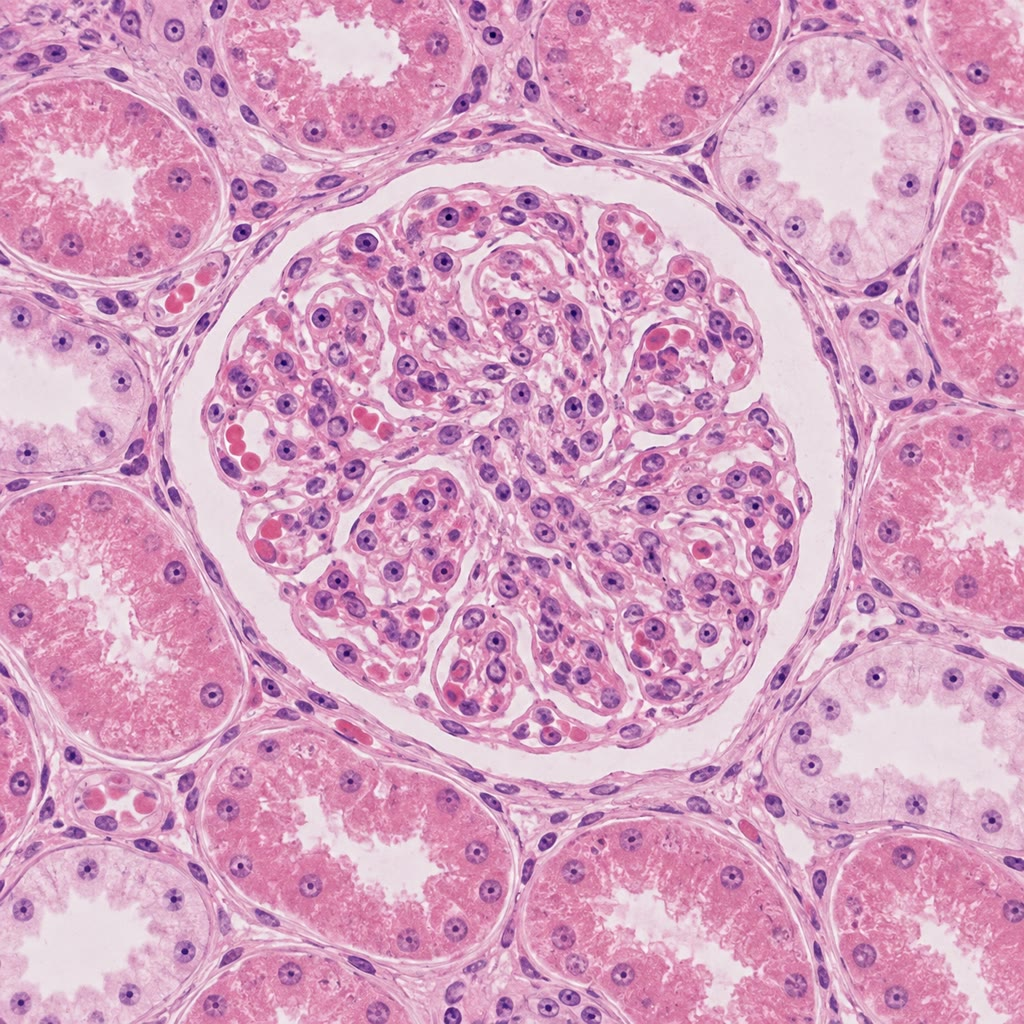
\includegraphics[width=0.46\linewidth]{images/book5/ai/b5-20-kidney-section.jpg}\hspace{0.04\linewidth}
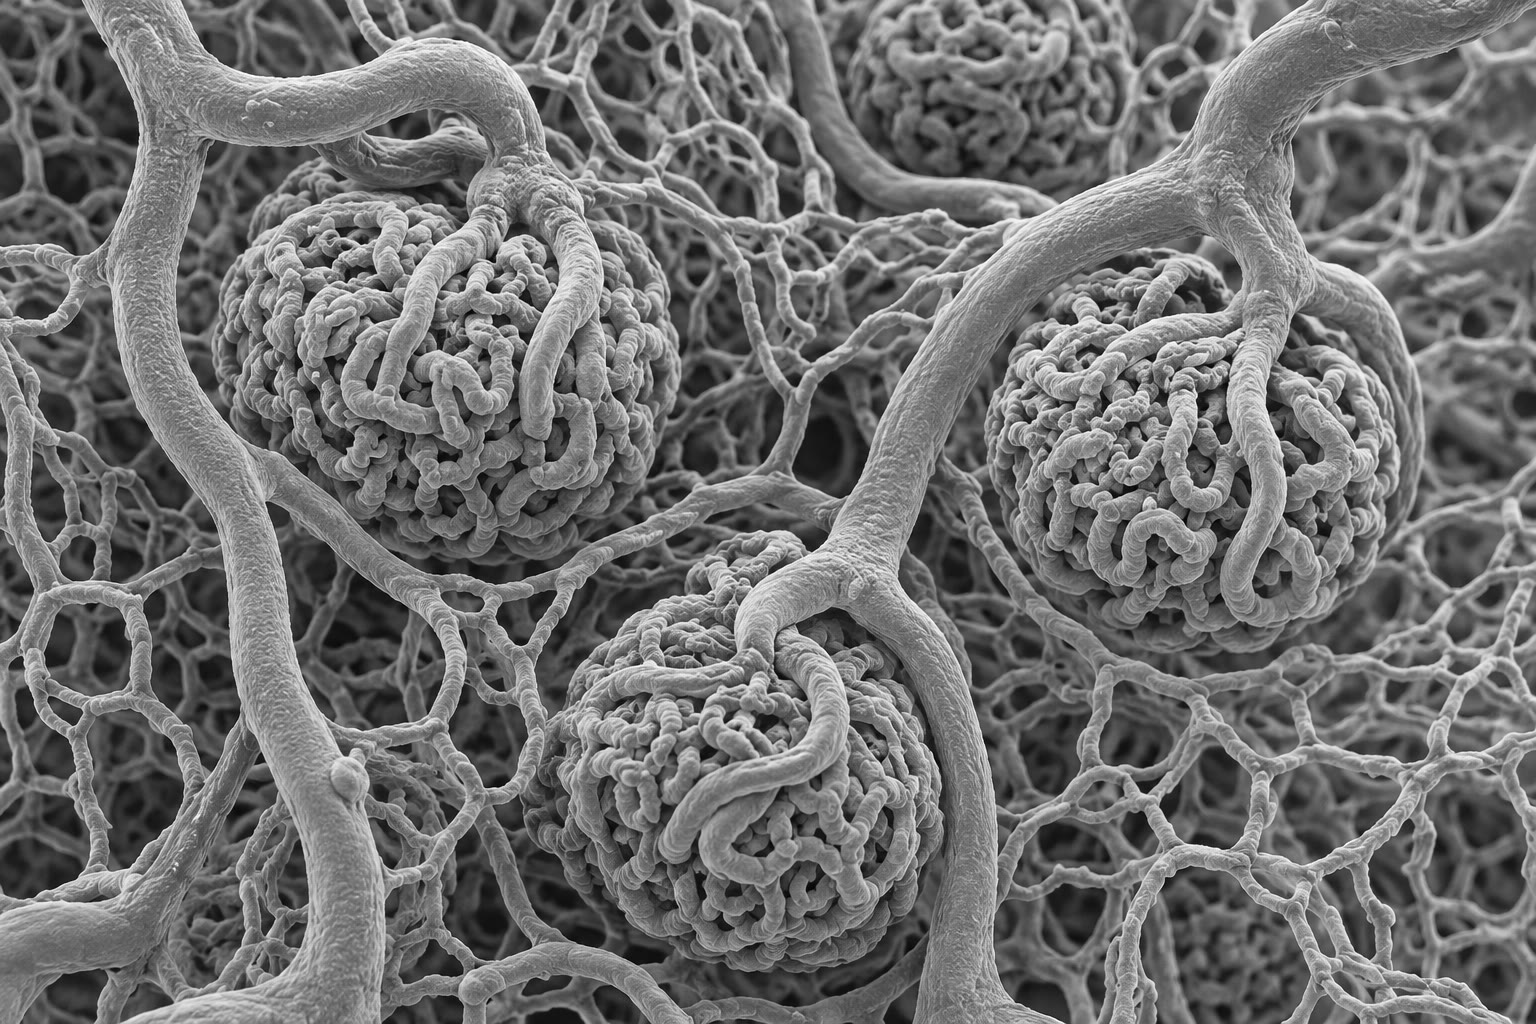
\includegraphics[width=0.46\linewidth]{images/book5/ai/b5-20-nephron-cast.jpg}

{\small À esquerda: córtex renal em corte --- um \omterm{def:b3:renal-osmoregulation:nephron}{glomérulo} em sua cápsula
entre os perfis dos túbulos proximais e distais. À direita: um molde
vascular do córtex, cada novelo um \omterm{def:b3:renal-osmoregulation:nephron}{glomérulo} com seus vasos aferente e
eferente entre os capilares peritubulares.}
\end{omfigure}

\section{Outros animais, outras soluções}

\begin{definition}[A osmorregulação entre os animais]\label{def:b3:renal-osmoregulation:comparative}
\index{túbulo de Malpighi}\index{glândula de sal}\index{célula de cloreto}\index{água metabólica}\index{espessura medular relativa}
Os peixes de água doce vivem num meio com um décimo da \omterm{def:b3:renal-osmoregulation:problem}{osmolaridade} de
seu sangue: a água inunda pelas brânquias, o sal vaza para fora, e eles
excretam uma urina copiosa e diluída e captam sal ativamente pelas
\emph{células de cloreto} das brânquias, sem nunca beber. Os teleósteos
marinhos, cujo sangue tem um terço da \omterm{def:b3:renal-osmoregulation:problem}{osmolaridade} do mar, perdem água
pelas brânquias, bebem água do mar e bombeiam o sal para fora pelas
mesmas células de cloreto, invertidas, mantendo escassa a urina; os
tubarões, em vez disso, mantêm o sangue isosmótico com o mar retendo
ureia (e óxido de trimetilamina para estabilizar suas proteínas contra
ela), e excretam o excesso de sal por uma glândula retal. As aves
marinhas e os répteis marinhos carregam \emph{glândulas de sal} acima dos
olhos, que secretam uma salmoura duas vezes mais salgada que o mar,
permitindo a um albatroz beber do oceano. Os insetos filtram por
\emph{túbulos de Malpighi} movidos por secreção ativa de potássio, e não
pela pressão sanguínea, e reabsorvem água no reto de modo tão completo
que as fezes de um besouro do deserto são secas. Entre os mamíferos, o
poder de concentração escala com o comprimento das alças em relação ao
tamanho do rim (a \emph{espessura medular relativa}): um castor alcança
\qty{500}{mOsm/L}, um humano \num{1200}, um camelo \num{3000}, o
rato-canguru \num{5500} --- o que lhe permite viver da \emph{água
metabólica} liberada quando seu alimento é oxidado, cerca de
\qty{0.6}{g} de água por grama de amido, com um focinho que recupera a
água de cada expiração por resfriamento em contracorrente.
\end{definition}

\begin{omfigure}
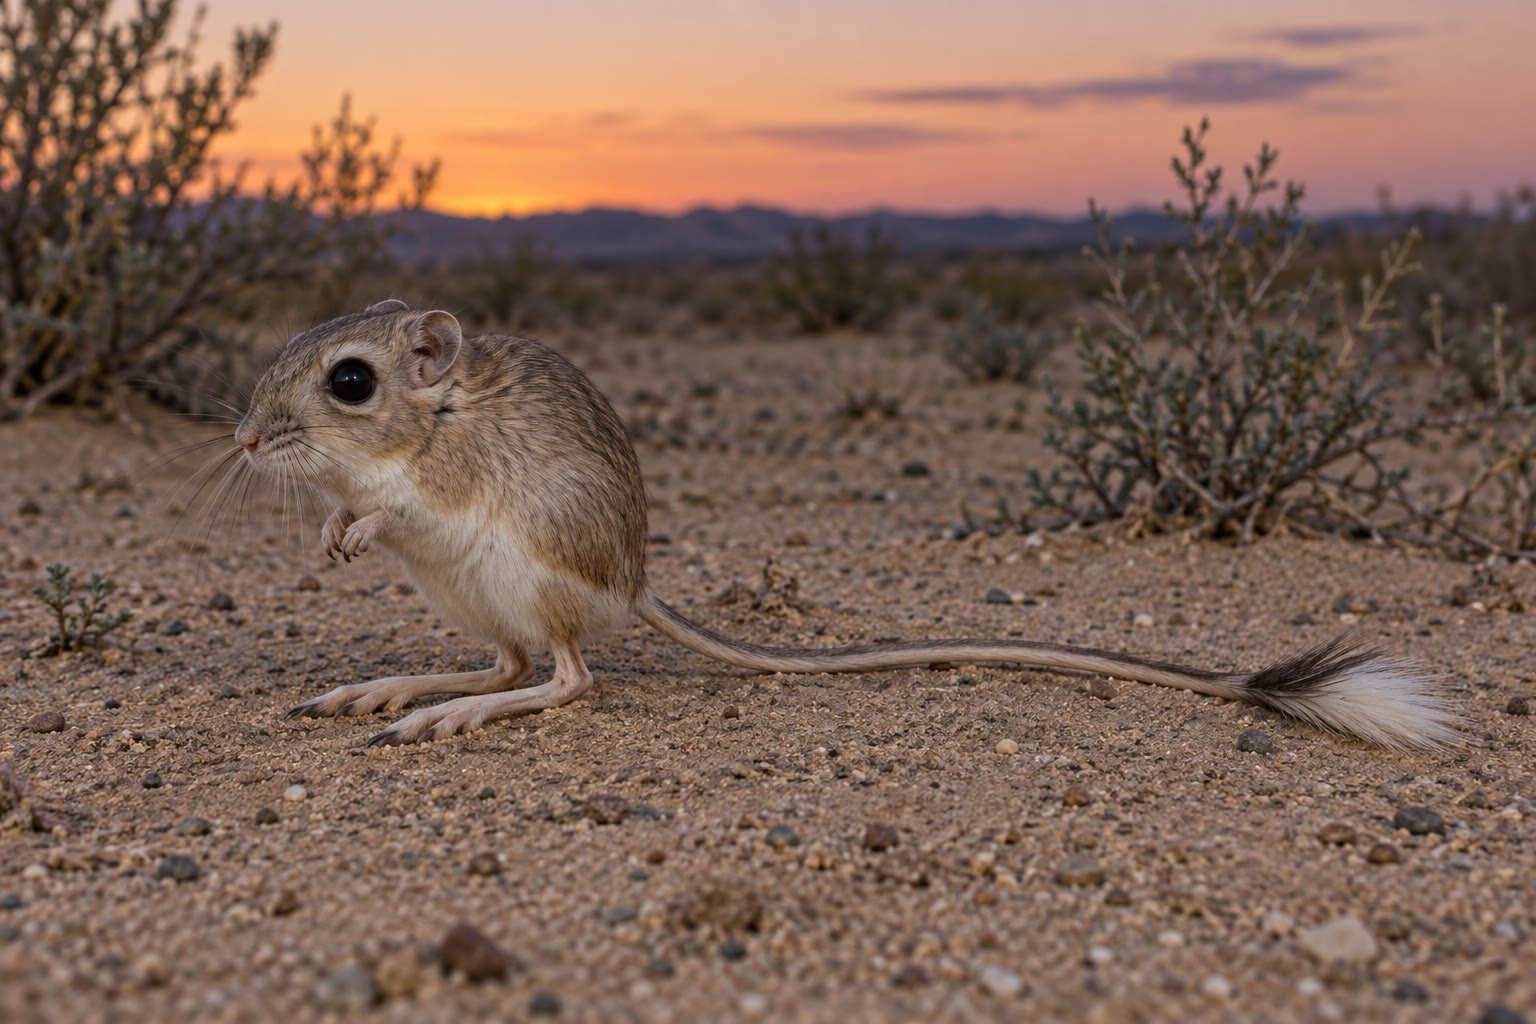
\includegraphics[width=0.56\linewidth]{images/book5/ai/b5-20-kangaroo-rat.jpg}

{\small Um rato-canguru, que nunca bebe: \omterm{def:b3:renal-osmoregulation:nephron}{alças de Henle} longas, uma urina
cinco vezes mais concentrada que a água do mar, um focinho frio que
condensa a água de cada respiração e uma dieta cuja oxidação faz toda a
água de que ele precisa.}
\end{omfigure}

\begin{remark}[O rim como problema de projeto]\label{rem:b3:renal-osmoregulation:design}
O rim dos mamíferos filtra quarenta vezes o volume plasmático por dia só
para retomar quase tudo: um projeto extravagante, cujo sentido é que
filtrar tudo e reabsorver seletivamente é mais simples que secretar
seletivamente todo resíduo que possa aparecer. Seu custo são os
\qty{7}{\%} do metabolismo de repouso gastos em bombear sódio de volta,
e sua vulnerabilidade é o filtro delicado, que falha devagar sob pressão
alta e glicose alta. Sua esperteza é a alça em contracorrente, um
dispositivo encontrado também nas bexigas natatórias dos peixes
profundos, nas pernas das aves pernaltas e nos focinhos dos roedores do
deserto, pelo qual uma diferença local pequena e acessível é empilhada
numa grande --- a mesma ideia, em cada caso, de que um gradiente pode ser
construído a partir do fluxo.
\end{remark}

\section{Exercícios}

\begin{exercise}[$\star$]\label{exo:b3:renal-osmoregulation:1}
Nomeie os segmentos do \omterm{def:b3:renal-osmoregulation:nephron}{néfron} em ordem e diga uma coisa que cada um
faz.
\end{exercise}

\begin{exercise}[$\star$]\label{exo:b3:renal-osmoregulation:2}
Defina clearance. Uma substância tem concentração plasmática de
\qty{2}{mg/mL}, concentração urinária de \qty{100}{mg/mL} e o fluxo de
urina é de \qty{1.5}{mL/min}. Calcule seu clearance e diga se ela é
reabsorvida, secretada ou nem uma coisa nem outra, se a TFG for de
\qty{120}{mL/min}.
\end{exercise}

\begin{exercise}[$\star$]\label{exo:b3:renal-osmoregulation:3}
Por que um peixe de água doce nunca bebe e um peixe marinho bebe sem
parar? O que fazem as brânquias em cada caso?
\end{exercise}

\begin{exercise}[$\star$]\label{exo:b3:renal-osmoregulation:4}
Qual é o \omterm{prop:b3:renal-osmoregulation:countercurrent}{efeito único} da \omterm{def:b3:renal-osmoregulation:nephron}{alça de Henle}, que ramo o produz, e por que os
dois ramos precisam diferir em sua permeabilidade à água?
\end{exercise}

\begin{exercise}[$\star\star$]\label{exo:b3:renal-osmoregulation:5}
Pressão do capilar glomerular de \qty{60}{mmHg}, espaço de Bowman de
\qty{18}{mmHg}, pressão oncótica plasmática de \qty{28}{mmHg} na
extremidade aferente subindo a \qty{35}{mmHg} na eferente. Calcule a
pressão líquida de filtração em cada extremidade e explique por que a
filtração pode cessar antes do fim do capilar. O que isso implica quanto
ao efeito do fluxo plasmático sobre a TFG?
\end{exercise}

\begin{exercise}[$\star\star$]\label{exo:b3:renal-osmoregulation:6}
O clearance de creatinina de um paciente é de \qty{40}{mL/min}. O sódio
plasmático é \qty{140}{mmol/L}, o sódio urinário \qty{70}{mmol/L} e o
fluxo de urina \qty{1}{mL/min}. Calcule a carga filtrada de sódio, a
excreção, a fração reabsorvida e o clearance do sódio.
\end{exercise}

\begin{exercise}[$\star\star$]\label{exo:b3:renal-osmoregulation:7}
Uma pessoa tem uma dieta que produz \qty{900}{mOsm} de soluto por dia e
consegue concentrar a \qty{1200}{mOsm/L}. Volume mínimo de urina? Se uma
doença renal baixar o máximo para \qty{400}{mOsm/L}, quanto ela precisa
beber para ficar em equilíbrio, contando \qty{0.9}{L} de perda
insensível?
\end{exercise}

\begin{exercise}[$\star\star$]\label{exo:b3:renal-osmoregulation:8}
Preveja o volume e a \omterm{def:b3:renal-osmoregulation:problem}{osmolaridade} da urina, o sódio plasmático e o
estado de sede em (a) diabetes insípido, (b) secreção inapropriada de
vasopressina por um \omterm{def:b3:cancer-biology:hallmarks}{tumor}, (c) excesso de \omterm{def:b3:renal-osmoregulation:controls}{aldosterona}, (d) uma dieta sem
sal algum por uma semana.
\end{exercise}

\begin{exercise}[$\star\star$]\label{exo:b3:renal-osmoregulation:9}
Calcule o \omterm{prop:b3:renal-osmoregulation:water}{clearance de água livre} para uma urina de \qty{100}{mOsm/L} a
\qty{6}{mL/min} e para uma urina de \qty{1000}{mOsm/L} a
\qty{0.6}{mL/min}, com o plasma a \qty{300}{mOsm/L}. Interprete cada um.
\end{exercise}

\begin{exercise}[$\star\star\star$]\label{exo:b3:renal-osmoregulation:10}
Modele a alça como $n$ estágios em que o líquido ascendente de cada
estágio está \qty{200}{mOsm/L} abaixo do interstício e o descendente
iguala o interstício, com o líquido entrando a \qty{300}{mOsm/L}.
Argumente que a \omterm{def:b3:renal-osmoregulation:problem}{osmolaridade} estacionária na curva pode se aproximar de
$300 +
200n$, de modo que o gradiente é limitado pelo comprimento da
alça e pelo \omterm{prop:b3:renal-osmoregulation:countercurrent}{efeito único} da bomba, e diga o que fixa $n$ fisicamente.
\end{exercise}

\begin{exercise}[$\star\star\star$]\label{exo:b3:renal-osmoregulation:11}
Um rato-canguru come \qty{5}{g} de semente seca por dia, \qty{80}{\%}
amido, oxidado a CO$_{2}$ e água (\qty{0.6}{g} de água por grama de
amido). Ele precisa excretar \qty{3}{mOsm} de soluto por dia a
\qty{5500}{mOsm/L}, e perde \qty{1.5}{g} de água por dia por evaporação
de um focinho que recupera \qty{70}{\%} da água de sua respiração.
Faça o balanço hídrico dele e diga se ele sobrevive sem beber.
\end{exercise}

\begin{exercise}[$\star\star\star$]\label{exo:b3:renal-osmoregulation:12}
A diálise faz o sangue passar de um lado de uma membrana e o dialisato
do outro, em contracorrente. Explique por que o fluxo em contracorrente
depura mais que o fluxo paralelo, estime o clearance de uma máquina que
remove ureia de \qty{300}{mL/min} de sangue com \qty{70}{\%} de
eficiência, e compare com dois rins ao longo de uma semana se a máquina
funcionar quatro horas três vezes por semana.
\end{exercise}

\section{Problema: Dezoito Baldes por Dia}

\begin{problem}[{Problema de fim de semana --- o filtrado de um dia
seguido do glomérulo à bexiga: as pressões de Starling, os clearances de
quatro substâncias, o limiar da glicose, o balanço hídrico da diluição
máxima até a água do mar e o balanço de um roedor do deserto, terminando
na TFG, no volume obrigatório de urina e na água líquida que um litro de
água do mar rende}]
\label{pb:b3:renal-osmoregulation:1}
Dados: $K_{f} = \qty{12.5}{mL/min/mmHg}$; $P_{\text{GC}} = \qty{55}{mmHg}$,
$P_{\text{BS}} = \qty{15}{mmHg}$, $\pi_{\text{GC}} = \qty{30}{mmHg}$.
Plasma: inulina \qty{0.5}{mg/mL}, creatinina \qty{0.01}{mg/mL}, ureia
\qty{5}{mmol/L}, glicose \qty{5}{mmol/L}, para-aminohipurato
\qty{0.02}{mg/mL}, Na$^{+}$ \qty{140}{mmol/L}, \omterm{def:b3:renal-osmoregulation:problem}{osmolaridade}
\qty{290}{mOsm/L}. Fluxo de urina \qty{1}{mL/min}: inulina
\qty{62.5}{mg/mL}, creatinina \qty{1.3}{mg/mL}, ureia \qty{250}{mmol/L},
glicose $0$, para-aminohipurato \qty{13}{mg/mL}, Na$^{+}$
\qty{100}{mmol/L}, \omterm{def:b3:renal-osmoregulation:problem}{osmolaridade} \qty{600}{mOsm/L}. Hematócrito $0.45$.
Glicose: $T_{m} =
\qty{375}{mg/min}$ (\qty{2.1}{mmol/min}). Soluto
diário \qty{600}{mOsm}; $U_{\max} = \qty{1200}{mOsm/L}$, $U_{\min} = \qty{50}{mOsm/L}$; perda insensível \qty{0.9}{L/d}; água do mar
\qty{1000}{mOsm/L}.

\medskip
\noindent\textbf{Parte I --- O filtro.}
\begin{enumerate}
  \item Calcule a pressão líquida de filtração e a TFG.
  \item Converta a TFG em litros por dia. Quantas vezes o volume
        plasmático (\qty{3}{L}) é filtrado?
  \item Calcule o clearance da inulina e compare com a TFG. Calcule o
        clearance da creatinina; por que ele é um pouco maior?
  \item Calcule o clearance do para-aminohipurato (o fluxo plasmático
        renal), o fluxo sanguíneo renal e a fração de filtração.
  \item A arteríola eferente se contrai, elevando $P_{\text{GC}}$ a
        \qty{60}{mmHg}. Nova TFG? Por que os fármacos que bloqueiam a
        angiotensina II baixam um pouco a TFG num rim sadio e protegem
        um rim diabético?
  \item Aparece proteína na urina a \qty{3}{g/d}. Que camada do filtro
        falhou, e o que acontece com a pressão oncótica plasmática e com
        os tecidos se isso continuar?
\end{enumerate}

\medskip
\noindent\textbf{Parte II --- Manejo.}
\begin{enumerate}[resume]
  \item Ureia: carga filtrada, excreção, fração reabsorvida e clearance.
  \item Sódio: carga filtrada por dia em moles e em gramas, excreção e
        fração reabsorvida. Quantos quilogramas de sal se perderiam em um
        dia se nada fosse reabsorvido?
  \item Glicose: carga filtrada em mmol/min e em gramas por dia; alguma
        é excretada? Com que glicose plasmática a carga filtrada alcança
        $T_{m}$ (o limiar)?
  \item Um diabético tem glicose plasmática de \qty{20}{mmol/L}. Glicose
        excretada por minuto e por dia em gramas, e o volume extra de
        urina se cada \qty{300}{mOsm} de glicose carregar \qty{1}{L} na
        concentração vigente. Explique a sede e a perda de peso do
        diabetes não tratado.
  \item Reabsorver sódio custa um ATP por três Na$^{+}$. Quantos moles de
        ATP por dia o rim gasta com o sódio, e quantos quilojoules
        (\qty{50}{kJ/mol})? Compare com um repouso de \qty{7}{MJ/d}.
  \item Explique por que o rim filtra e reabsorve em vez de secretar cada
        resíduo, em termos do que o túbulo precisaria reconhecer.
\end{enumerate}

\medskip
\noindent\textbf{Parte III --- Água.}
\begin{enumerate}[resume]
  \item Clearance osmolar $U_{\text{osm}}V/P_{\text{osm}}$ a partir dos
        dados, e o \omterm{prop:b3:renal-osmoregulation:water}{clearance de água livre}. A pessoa está conservando ou
        eliminando água?
  \item Volume mínimo de urina para o soluto diário; máximo (em
        $U_{\min}$); a necessidade total de água por dia no mínimo, com
        a perda insensível.
  \item Bebe-se um litro de água do mar. Quanta urina é necessária para
        excretar seu sal em $U_{\max}$, e qual é o ganho líquido de água
        antes de contar o soluto do próprio dia? E depois?
  \item A vasopressina está ausente (diabetes insípido) e a urina fica em
        $U_{\min}$. Volume diário de urina para o mesmo soluto, e a água
        que precisa ser bebida a cada dia para manter o equilíbrio.
  \item Cerveja a \qty{20}{mOsm/L}: quanto se pode beber por dia antes
        que o rim, em $U_{\min}$, já não consiga excretar a água? (A água
        em excesso do que o soluto consegue carregar em $U_{\min}$ se
        acumula.)
  \item Depois de uma noite sem água a \omterm{def:b3:renal-osmoregulation:problem}{osmolaridade} plasmática é de
        \qty{298}{mOsm/L}. Em quantos por cento ela subiu, e o que faz o
        hipotálamo? Estime o déficit de água se a água corporal total é
        de \qty{42}{L} e o soluto não mudou.
  \item Explique por que um maratonista que bebe \qty{6}{L} de água
        enquanto sua sal pode desenvolver um sódio plasmático
        perigosamente baixo, e o que o rim precisaria fazer para
        impedi-lo.
\end{enumerate}

\medskip
\noindent\textbf{Parte IV --- O deserto.}
\begin{enumerate}[resume]
  \item Um rato-canguru excreta \qty{3}{mOsm} por dia a
        \qty{5500}{mOsm/L}. Volume de urina? Compare com o volume de que
        um rim humano precisaria para o mesmo soluto em seu próprio
        máximo.
  \item Seu alimento rende \qty{2.4}{g} de \omterm{def:b3:renal-osmoregulation:comparative}{água metabólica} por dia e ele
        perde \qty{1.6}{g} respirando e \qty{0.3}{g} nas fezes. Faça o
        balanço com a urina da questão 20.
  \item Um camelo concentra a \qty{3000}{mOsm/L} e tolera perder
        \qty{25}{\%} de sua água corporal. Para um camelo de
        \qty{500}{kg} com \qty{65}{\%} de água, quanto ele pode perder, e
        quantos dias isso cobre a uma perda de \qty{5}{L/d}?
  \item Uma ave marinha come \qty{200}{g} de peixe e bebe \qty{100}{mL}
        de água do mar por dia, ingerindo \qty{150}{mmol} de NaCl. Sua
        \omterm{def:b3:renal-osmoregulation:comparative}{glândula de sal} secreta a \qty{800}{mmol/L}. Quanta salmoura ela
        produz, e por que a glândula é melhor que o rim (que nas aves
        concentra apenas a \qty{600}{mOsm/L}) para isso?
  \item Um peixe de água doce de \qty{100}{g} ganha \qty{30}{\%} de sua
        massa corporal em água por dia pelas brânquias. Quanta urina ele
        precisa fazer, em que \omterm{def:b3:renal-osmoregulation:problem}{osmolaridade} em relação ao seu sangue, e o
        que aconteceria com seu sal sem a captação ativa?
  \item Resuma: a TFG (questão~1), o volume obrigatório de urina
        (questão~14) e a água líquida de um litro de água do mar depois
        de contado o soluto do dia (questão~15).
\end{enumerate}
\end{problem}
